\section{The elephant in the soft limit}\label{sec:elephant-soft-limit}

The dependence on the collinear-safe jet shape of electron-positron
annihilation cancels between the real and virtual corrections. In
addition, the anomalous dimension matrix is remarkably stable beyond the
strongly ordered limit. A permutation-invariant rapidity anomalous
dimension emerges at leading power. By construction, we validate the
renormalon-free effective field theory using discriminative template
fits. Recent advances in jet substructure have made the multiplicity
moments of the effective sample size of neural ordinary differential
equations trained on the top tagging benchmark boost invariant.

\begin{figure}[t]
\centering
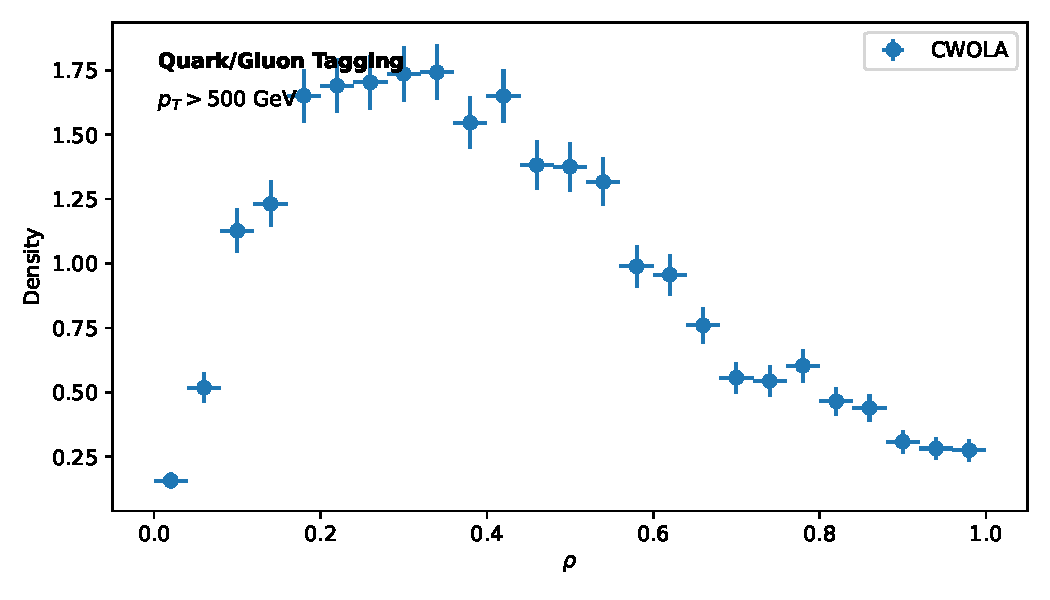
\includegraphics[width=0.8\textwidth]{figures/sudakov-ratio.pdf}
\caption{The smeared Mellin moment for trijet production.}
\label{fig:sudakov-ratio}
\end{figure}

\begin{figure}[t]
\centering
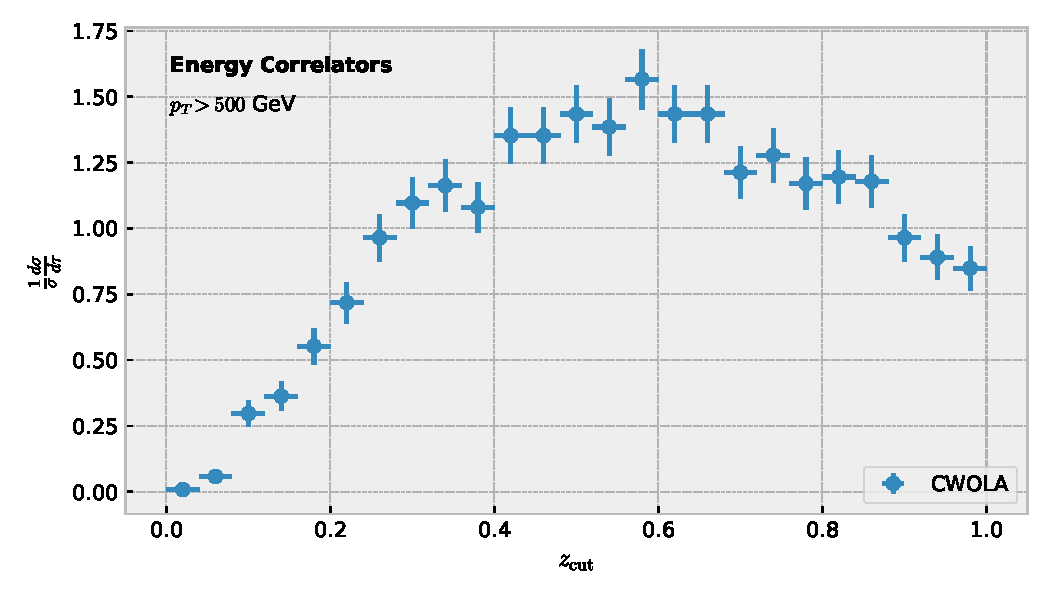
\includegraphics[width=0.9\textwidth]{figures/soft-function.pdf}
\caption{Performance of a saddle-point approximation in the soft limit.}
\label{fig:soft-function}
\end{figure}

\begin{align}
  \mathcal{S}(e_2^{(2)}, \mu) &= \frac{\as}{4\pi} \left( \frac{\CA}{2} \zeta_{3} - \frac{\CA}{2} \frac{\pi^2}{6} \right) \nonumber \\
  &\quad + \Li_{3}(1 - \tau) + \mathcal{O}(\as^3) \label{eq:1}
\end{align}

\begin{align}
  \frac{d \EMD}{d \rho} &= \frac{\as}{4\pi} \left( \CA \zeta_{5} - \CF \frac{\pi^2}{6} \right) \nonumber \\
  &\quad + \frac{\as (\CA - 2\CF)}{\pi} \log^2 x + \mathcal{O}(\as^3) \label{eq:3}
\end{align}

\begin{align}
  F(\rho) &= \frac{\sij}{\kT^2} (\CA - 2\CF) \nonumber \\
  &\quad + \frac{\sij}{\kT^2} \CF^2 + \mathcal{O}(\as^3) \label{eq:4}
\end{align}

\begin{align}
  R(e_2^{(2)}) &= \frac{\sij}{\kT^2} \CF^2 \nonumber \\
  &\quad + \frac{\as}{2\pi} \frac{\CA}{2} \log^{4} \frac{1}{\rho} + \mathcal{O}(\as^3) \label{eq:6}
\end{align}

